\subsection{Basic Idea of mmprof}

\begin{figure}[!ht]
\centering
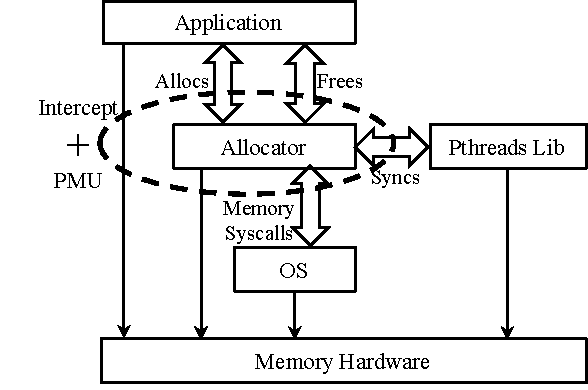
\includegraphics[width=3in]{figures/overview}
\caption{Basic idea of \texttt{mmprof}.\label{fig:basicidea}}
\end{figure}

\MP{} is designed as a drop-in library that can be simply linked to applications (and allocators) with the preloading mechanism, which does not require the change or the re-compilation of applications and allocators.

\MP{} aims to discover common factors of an  allocator as discussed in Section~\ref{sec:factors}. Since allocators provide the same APIs to applications, invoke a limited set of system calls, and employ the similar thread synchronization primitives, \MP{} intercepts the interactions between an allocator and other components of the system. Such components include the application, the OS, and the pthreads library. The basic idea of \MP{} is shown as Fig.~\ref{fig:basicidea}. The interception allows \MP{} to collect the information of each interaction, and report the averaged number in the end. 

In order to collect the runtime of each interaction, \MP{} further employs the Time-Stamp Counter with the RDTSC instruction~\cite{coorporation1997using, weaver2013linux}. The Time-Stamp Counter is a hardware register available in X86 computers, which tracks the number of cycles since the reset time. The RDTSC instruction has two advantages over a system call, such as \texttt{gettimeofday}. First, its overhead is much lower than invoking a system call, typically in the level of  cycles~\cite{rdtscoverhead}, instead of thousands of cycles. Second, it provides the information in the granularity of cycles, which is much finer than the microseconds that a system call can provide~\cite{pitfallsrdtsc}. With the RDTSC instruction, \MP{} obtains the timestamp before and after each operation, and uses the difference of timestamps as the runtime of a specific operation. \MP{} is able to measure the averaged runtime of each system call, each synchronization, and each memory management operation. 

However, the invocation information alone cannot  explain the design issue inside and an allocator's application friendliness. \MP{} further employs hardware Performance Monitoring Units (PMU) to collect the information of memory accesses and hardware events. As shown in Fig.~\ref{fig:basicidea}, \MP{} focuses on accesses and events for both inside and outside of memory management operations. The PMU hardware is ubiquitous in modern architectures~\cite{AMDIBS:07, IntelArch:PEBS:Sept09, armpmu}, and has been  employed to sample memory accesses or hardware-related events~\cite{DBLP:conf/sc/ItzkowitzWAK03, ibs-sc, ibs-pact, Sheng:2011:RLN:1985793.1985848, LASER, Cheetah}.
%, such as memory loads and stores, hardware instructions, cache misses, and TLB misses
For each sampled memory access, PMUs provides the type of an access (load or store), and instruction position, timestamp, and memory address. \MP{} utilizes sampled memory accesses to identify cache contention effect, false sharing effect, cache utilization rate, and page utilize rate, as discussed in Section~\ref{sec:profilefriendliness}. PMUs also reports the number of instructions, page faults, TLB misses, and cache misses for inside and outside of allocation. Therefore, \MP{} helps programmers identify particular design issues inside an allocator. 


Overall, \MP{} focuses on the metrics of an  allocator and application friendliness. It  reports all metrics listed in Table~\ref{table:alldata}, by employing either RDTSC or PMUs techniques. The data, when combined together, explains the performance, scalability, memory consumption of an allocator. It also helps predict the potential issue of an allocator. 

\subsection{Technical Challenges}

As described above, \MP{} employs hardware PMUs, time-stamp counters, and simple counters together to perform the profiling. But there exist some technical challenges as follows. 

The first and the most important challenge is the \textbf{overhead challenge}, where a careless design may impose up to 100 $\times$ overhead based on our development experience. The huge overhead could be unaffordable even for development phases. More importantly, the significant overhead may also skew the evaluation results unnecessarily. Therefore, \MP{} should design some efficient mechanisms to perform the collection, such as three-level lookup mechanism as shown in Section~\ref{sec:profilefriendliness}. 

The second challenge is collect some metrics precisely, such as memory blowup, cache utilization rate, passive/active false sharing. Some of these metrics, such as memory blowup, are not evaluated quantitatively, although they have been proposed long time ago. \MP{} designs some specific . 

The third challenge is to balance the efficiency, interference, and correctness. 

Statistically. 

The fourth challenge is to deal with the thread migration caused by the allocator. 

 

Other challenges come from the adaption to different allocators. Specific issues include the following ones: (1) How to obtain the specific details of different allocators, such as size class information, type of allocator, metadata size information? (Section~\ref{sec:understandingallocators}) (2) How to design a general but fast lookup mechanism for different allocators? (3) How to profile kernel-contention for allocators?



% Comparing to the method of utilizing system calls, such as \texttt{gettimeofday()}, the RDTSC instruction has two advantages. First, the overhead is much lower than issuing a system call, typically around 25-35 cycles~\cite{rdtscoverhead}. Second, it provides a high-resolution timer, with the granularity of cycles, which is much finer than traditional system calls~\cite{pitfallsrdtsc}. For instance, the system call \texttt{gettimeofday} could only provide the microsecond granularity, which is too coarse for measuring the performance of system calls or synchronization overhead.  





